\subsection{IMU Testing}
The PmodNAV IMU is a small device that was directly connected to the ZedBoard's Pmod connector. As such, it required no external power source or other intermediate connections.

\subsubsection{Communication Testing}
With the rangefinder connected to the ZedBoard's PS MIO Pmod, JE, the PmodNAV IMU required an Extended MIO Pmod so that it was able to be controlled by the PS. As such, the SPI pins were routed to the JD Pmod. Since the only slave this project used on the PmodNAV was its magnetometer, the slave select and register settings were adjusted accordingly, as discussed in Section \ref{imu_settings}. To choose the magnetometer and deselect the accelerometer/gyroscope and barometer, the magnetometer's slave select was brought low for each SPI transfer while the other two were left high. The behavior of Pmod JD's pins were observed with an oscilloscope during an SPI transfer. It was observed that as soon as the magnetometer's slave select line was asserted there was unidentified behavior with all of the other pins. Since the PmodNAV was disconnected this issue was thought to be with routing the SPI pins to EMIO incorrectly, so it was decided to test the SPI transfer via Pmod JE.
\par
The pins were re-routed to the MIO Pmod JE and similar undefined functionality was observed when the magnetometer's slave select line was asserted. The ZedBoard's SPI errata was investigated until AR\# 47511 was found, which describes an unresolved issue in the MIO interface where the SPI controller resets itself when slave select 0 signals asserts \cite{zedboardErrata}. Since this issue affected the PS SPI controller itself, this errata was also the cause of the EMIO's undefined behavior.
\par
To avoid the problems with SPI on the ZedBoard, I\textsuperscript{2}C was attempted next, since the PmodNav supports I\textsuperscript{2}C communication. I\textsuperscript{2}C was routed to Pmod JD. Communication with the PmodNAV's magnetometer was tested through I\textsuperscript{2}C, but it was learned that the magnetometer was inaccessible through the I\textsuperscript{2}C bus. As such, SPI was the only option and needed to be implemented.
\par
The SPI pins were again routed to Pmod JD. To avoid the errata, slave select 1 was assigned to the magnetometer. The other two slave select pins were routed away from Pmod JD so that they were not used in any manner. Instead, two GPIO pins were used and configured as pull-ups so that these pins idled high and never had to be written to. This setup was configured in Vivado's Synthesis tab, as shown in Figure \ref{emio_config}. 

\begin{figure}[H]
	\centerline{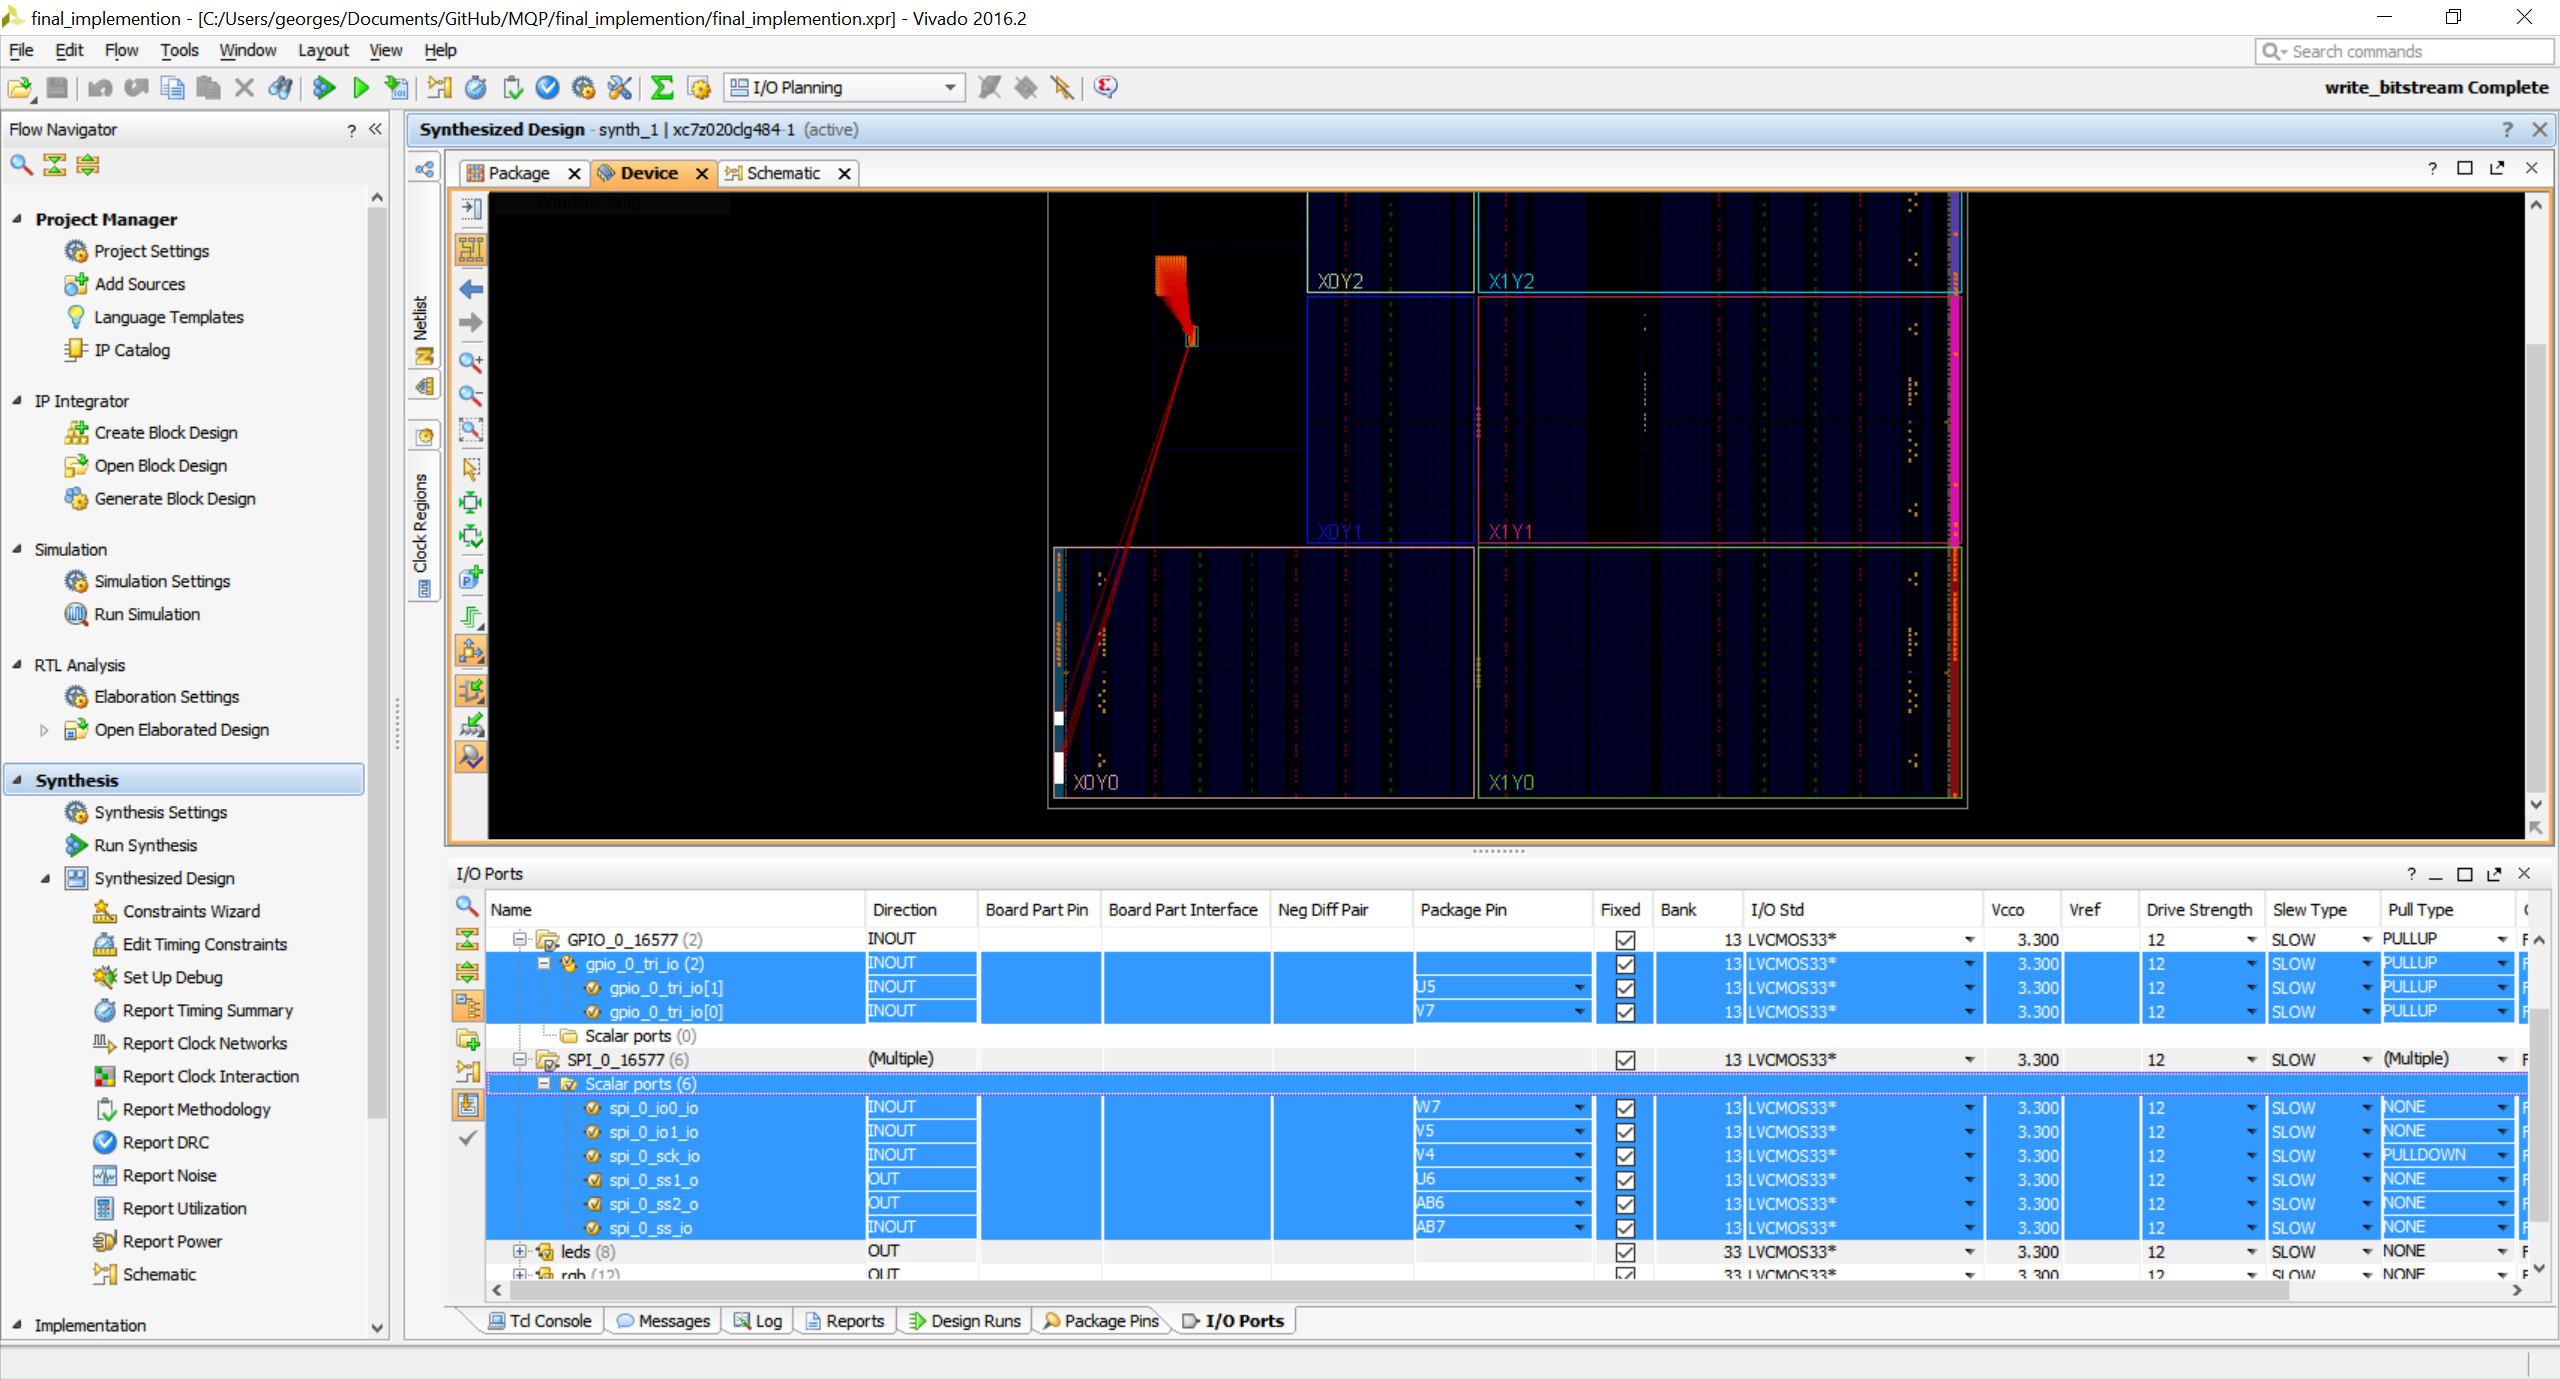
\includegraphics[width=1.1\textwidth]{editing_emio_pins.png}}
	\caption{EMIO SPI Configuration for PmodNAV}
	\label{emio_config}
\end{figure}

With this configuration a waveform similar to those shown in Figures \ref{magnetometer_spi} and \ref{multiple_reads} were observed, indicating that the errata was avoided and the the ZedBoard's SPI waveforms were accurate. The PmodNAV was connected to the ZedBoard and successful communication was observed on the oscilloscope, as shown in Figure \ref{OTPHJ}.

\begin{figure}[H] 
	\begin{subfigure}{1\textwidth}
	\centering
		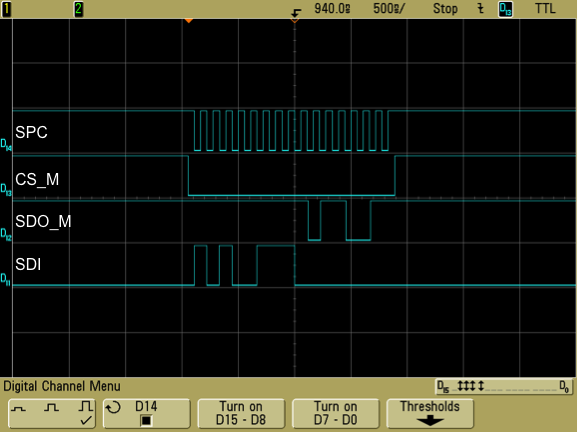
\includegraphics[width=0.75\linewidth]{magSingleRead_label.png}
		\caption{IMU Magnetometer Single Read Operation}
	\end{subfigure}
	\begin{subfigure}{1\textwidth}
	\centering
		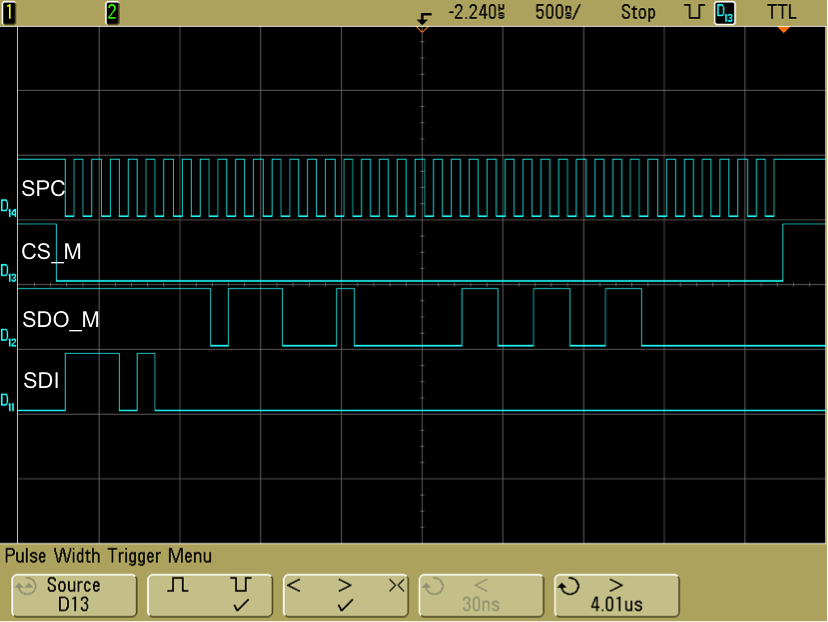
\includegraphics[width=0.75\linewidth]{magMultRead_label.png}
		\caption{IMU Magnetometer Multiple-Byte Read Operation}
	\end{subfigure}
	\caption{Successful IMU Communication via EMIO SPI}
	\label{OTPHJ}
\end{figure}

\subsubsection{Data Testing}
The IMU's data was tested by transmitting it via UART after its data processing. By the end of its data processing, the magnetometer's data was transformed into a compass heading. The ZedBoard's UART was routed to USB UART and connected to a serial console. The sensor suite was rotated, and the compass heading was observed. The results were inaccurate and inconsistent until the sensor suite was moved as far from the lab bench as the wires allowed. The PmodNAV was a very sensitive piece of equipment that was susceptible to electromagnetic interference, in this case most noticeably by the ZedBoard's own power supply. Once the device was further away from the lab bench, accurate and repeatable compass headings were observed.

\subsubsection{Interfacing with the ADIS16375 IMU}
Although this project ultimately interfaced with the PmodNAV IMU, this was not the first IMU that communication was attempted with. Originally, the ADIS16375 Six Degrees of Freedom Inertial Sensor, shown in Figure \ref{adis16375}, was intended to be used in the sensor suite.

\begin{figure}[H]
	\centerline{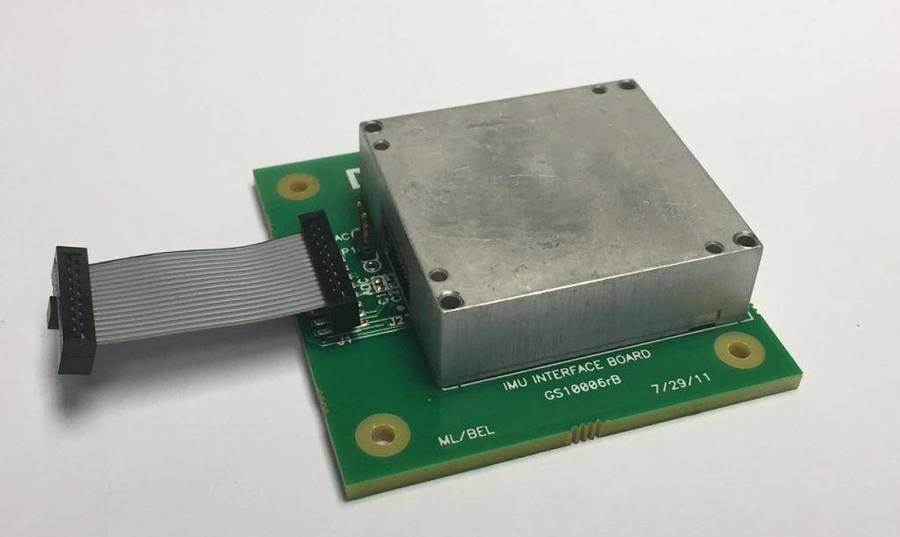
\includegraphics[width=.7\textwidth]{adis16375.jpg}}
	\caption{The ADIS16375 Six Degrees of Freedom Inertial Sensor \cite{adisBreakout}}
	\label{adis16375}
\end{figure}

The ADIS16375 IMU was a highly sensitive, heavy duty device. It had a tri-axis gyroscope, a tri-axis accelerometer, and a temperature sensor, had onboard functionality to calculate delta-angle and velocity, and used SPI communication. Although the ADIS16375 did not have a magnetometer, its gyroscope's sensitivity combined with its sample rate and onboard delta-angle calculation made it perfect to account for rotation. However, communication was not able to be established with it. There was no way to test the ADIS16375 so its functionality could not be confirmed in any manner. Instead, the PmodNAV was implemented as a quicker and simpler solution.




